\documentclass[letterpaper]{article}

\usepackage{hyperref}
\usepackage{tikz}
\usepackage{listings}
\usepackage{amsfonts}

\definecolor{code_green}{rgb}{0, 0.6, 0}

\lstdefinestyle{Code_Style}{
    basicstyle=\ttfamily,
    commentstyle=\color{code_green},
    keywordstyle=\color{blue},
    breakatwhitespace=false,
    breaklines=true,
    keepspaces=true,
    numbers=left,
    showspaces=false,                
    showstringspaces=false,
    showtabs=false,
    tabsize=4
}

\lstset{style=Code_Style}

\title{Amazon Delivery Truck Simulation}
\author{Hanna Butt \thanks{HFB352, \href{mailto:hannaf2020@gmail.com}{hannaf2020@gmail.com}} \and Ashton Cole \thanks{AVC687, \href{mailto:ashtonc24@utexas.edu}{ashtonc24@utexas.edu}} \and Kelechi Emeruwa \thanks{KEE688, \href{mailto:kelechi@utexas.edu}{kelechi@utexas.edu}}}
\date{\today}

\begin{document}
    \maketitle

    \begin{abstract}
        Summary of whole paper. Note that this is not an introduction or context, but a summary.
    \end{abstract}

    \section{Introduction}
    \label{section:Introduction}
    Imagine that a delivery company has a series of orders that it needs to fulfill. It has a truck that can stop at each address and make the delivery. The company naturally wants to save on time and fuel costs, so it tries to find the shortest path from its warehouse to cover all of the stops. This is the basic premise of the Traveling Salesman problem. Our team chose to solve it for our final project in COE 322: Scientific Computation at the University of Texas at Austin for the fall of 2022.
    
    In Section \ref{section:Methodology} we discuss the algorithm that we used to solve the simple Traveling Salesman Problem, and expansions upon it to construct our final program. In Section \ref{section:Results}, we display the outcomes of several test scenarios and discuss the results. Finally, in Section \ref{section:Conclusion}, we offer our final thoughts and reflect on ethical considerations. However, we will first further define the problem for our purposes and apply some limitations and assumptions in the following subsections.

    \subsection{Perfect is the Enemy of Good}
    \label{subsection:Perfect_is_the_Enemy_of_Good}
    One could simply test each of the $n!$ combinations of a list of $n$ addresses to fund the one with the shortest total distance, but with 4 stops this becomes quite tedious, and after that nearly untenable. A computer could solve this faster, but the problem still becomes very computationally expensive at a factorial rate. The preferable alternative is to use algorithms to find good and better paths, significantly cutting down on calculations. Perhaps it will neglect the perfect solution, but in a world with finite resources, we have to make the trade-off to settle for less. The algorithms which we employ, detailed in Section \ref{section:Methodology} reflect this.

    \subsection{Earth is Flat}
    \label{subection:Earth_is_Flat}
    We also have to restrict the definitions of an address and the distance between addresses. Since this project is intended to focus on algorithms, not a turn-key solution for use in the real world, addresses are represented with Cartesian coordinates on a two-dimensional Euclidian plane. Distances are assumed to be Euclidian, i.e. ``as the bird flies,'' with travel times proportional thereto. The distance could alternatively be defined as the ``Manhattan Distance,'' i.e. the distance along a perfect rectilinear street grid. Although using real-world geographic data considering road layouts, speed limits, real-time traffic data, and Earth's curvature would be more realistic, it would add significant complexity to our implementation without contributing much to the core principles of the solution.

    \subsection{TODO}
    MORE DEFINITIONS HERE: deliver by date, multiple days, multiple trucks

    \section{Methodology}
    \label{section:Methodology}
    % Notes: Talk about how we're solving the problem (C++, TACC super computer, icpc compiler) and how the program works (e.g. reads in text file, spits out text file). Then go into the development process/timeline (we started simple with address/list classes, tested functionality, and then expand it a bit)

    To approach this problem, we wrote a library and scripts in C++. These were compiled with GNU's \verb|g++| on our local machines and Intel's \verb|icpc| on the Texas Advanced Computing Center's ISP supercomputer. These scripts are outlined below.
    \begin{itemize}
        \item \verb|traveling_salesman.h|: a header file for our TravelingSalesman library, defining all of the objects and algorithms used in the project
        \item \verb|traveling_salesman.cpp|: an implementation file
        \item \verb|tester.cpp|: a script which tests the functionality of our TravelingSalesman library and generates TikZ code for figures displayed in this report; this script is compiled as \verb|tester.exe|
        \item \verb|deliveries_generator.cpp|: a script which generates \verb|.dat| files containing lists of orders to be processed by \verb|delivery_truck_simulation.exe|; this script is compiled as \verb|deliveries_generator.exe|
        \item \verb|delivery_truck_simulation.cpp|: a script which represents a hypothetical final product for use in industry, as described in Section \ref{subsection:Developing_the_Final_Product}; this script is compiled as \verb|delivery_truck_simulation.exe|
    \end{itemize}

    We began our project by writing the header and implementation files, coupled with tests in our tester file. After we confirmed that all of our objects and algorithms functioned as expected, we designed a main program to best parallel a real world application of solving the Traveling Salesman Problem. The structures and algorithms that we developed are further detailed in this section.

    In Section \ref{subsection:Object-Oriented_Structure}, we outline the structure of the classes that we used to represent and solve the problem. In Section \ref{subsection:Traveling_Salesman_Problem}, we describe the algorithms we used to solve the simple Traveling Salesman Problem. In Section \ref{subsection:Multiple_Traveling_Salesmen_Problem}, we describe the expansion of the problem to account for optimizing multiple delivery routes. Finally, in Section \ref{subsection:Developing_the_Final_Product}, we describe how we combined our algorithms into a final product for a hypothetical user.

    \subsection{Object-Oriented Structure}
    \label{subsection:Object-Oriented_Structure}
    Our scripts took advantage of C++'s object-oriented capabilities to organize the problem. This section provides a brief overview; the contents of these classes are not described exhaustively.
    
    Each delivery stop is represented by an \verb|Address| object, which has two-dimensional integer Cartesian coordinates \verb|i| and \verb|j| representing the location of the address, an an integer \verb|deliver_by| which describes the day by which the order is supposed to be delivered, or the stop passed-by. The class can also calculate the distance to other \verb|Address|es, using either the Euclidian distance $\sqrt{i^{2} + j^{2}}$ or Manhattan distance $|i| + |j|$. In our implementation, we use the Euclidian distance, but it could easily be replaced with another formula.

    A list of \verb|Address|es is represented by an \verb|AddressList| object, which holds the objects in a \verb|std::vector<Address>| instance variable called \verb|address_list|. This class can add, remove, and rearrange \verb|Address|es. It does not accept duplicate \verb|Address|es, i.e. those with the same coordinates. If the user attempts to add an order to the same \verb|Address| with different \verb|deliver_by| due dates, then the lesser value is accepted. This parallels orders being combined in real life. Note that the preference for the earlier date is based on the assumption that at the time that the \verb|Address|es are added to the \verb|AddressList|, they are available to be delivered.

    The \verb|Route| class extends the \verb|AddressList| class by including a \verb|hub| instance of type \verb|Address|. This represents the starting and ending point of the \verb|Route|. This class contains several functions to solve variants of the Traveling Salesman problem.

    \subsection{Traveling Salesman Problem}
    \label{subsection:Traveling_Salesman_Problem}

    Having developed a strong Object-Oriented skeleton we can 
    explore algorithms to address the Traveling Salesman Problem. 
    An intuitive approach we could adopt is called the 
    \emph{greedy algorithm} also known as the \emph{nearest neighbor algorithm}. \cite[p.~458]{cite:eijkhout2022}  
    The greedy algorithm works to develop an optimal route by traversing (from a starting point)  
    to the next closest point in a list of points until all points in the list have been visited.
    To achieve this optimal route, the greedy algorithm must 
    determine which point is closest to the current point at each iteration.
    This can be accomplished with the help of our \emph{index\textunderscore closest\textunderscore to()}
    method. Now we can iterate through the list of addresses 
    and at each iteration calculate the next closest address 
    until we have visited all the addresses in our list. To 
    prevent visiting the same address more than once, we can 
    make another list, and pop elements from our current list 
    into our new (optimized) list. Since we call our 
    \emph{index\textunderscore closest\textunderscore to()} 
    method n times (where n is the length of our address list) 
    and the method itself has a time complexity of O(n) we 
    arrive at a Big-O time complexity of O(n\textsuperscript{2}) for this 
    greedy algorithm . The figure below illustrates the 
    effect our greedy algorithm has on developing a more 
    optimized route.     \ref{figure:sortdemo}.
    \begin{figure}[h]
        \caption{insert improvement from greedy alog }
    \end{figure}
    The improvements from the greedy algorithm seem to suggest that it 
    will play an important role in developing our Amazon route scheduling 
    algorithm. On the other hand, additional testing demonstrates how 
    the greedy algorithm alone can fail to provide the most accurate solutions:
    
    \begin{figure}[h]
        \caption{ insert deficiency of greedy algorithm }
    \end{figure}
    
    Although this deficiency may seem minimal with a few routes, at scale , 
    the costs incurred due to longer distances traveled and longer delivery 
    times may prove to be a great burden for Amazon, therefore we'd like to 
    explore better methods. One approach we can adopt is based on the opt-2 
    heuristic. The opt-2 heuristic suggests that optimal routes are generally 
    not “entangled” (i.e no intersections). Therefore, if we can work to “detangle” 
    a given list of points we can find its optimal path. Both pathes can be seen 
    in the figure below. 

    \begin{figure}[h]
        \caption{ ** insert entangled vs detangled route and its total distance. }
    \end{figure}

    Rather than aim to algorithmically identify the intersections in a given path, 
    we can try to “detangle” a path by reversing segments of it and checking to 
    see if such a modification generates a more optimal path. The figure below 
    shows how this is done visually.

    \begin{figure}[h]
        \caption{ ** insert single pass of reversage of a path }
    \end{figure}

    To implement this in code, we employ the strategy in Listing \ref{lst:opt2_algorithm}.

    % need to fix, there's a better package than fbox that 
    % needs looking into
    \begin{lstlisting} [
        caption=opt2 Algorithm,
        label={lst:opt2_algorithm}
    ]
For all possible segments in our path:
    Make the new path:
        Original start + reversed segment + original end 
        If new path is shorter keep it\end{lstlisting}

    In code this equates to:
    \begin{lstlisting}[
        language=C++
    ]
Route Route::opt2(){
    AddressList address_list(address_vec);
    double current_length = address_list.length();
    for (int m=1 ; m<address_list.size(); m++){
        for (int n=0; n <= m; n++){
            AddressList new_list(address_list.reverse(n, m+1));
            if ( new_list.length() < address_list.length() ){        
                address_list = new_list;
                current_length = new_list.length();
            } 
        }
    }
    Route new_route(address_list, hub);
    return new_route;
}
\end{lstlisting}

    In this implementation, we utilized the \emph{reverse()} method 
    from the C++ standard library reverses a given segment of a vector 
    in place. Below we compare the results from our greedy algorithm 
    with that of our opt-2 algorithm:

    \begin{figure}[h]
        \caption{compare greedy w/opt 2 
        (use previous greedy deficiency example too)}
    \end{figure}

    The opt-2 algorithm seems to be a reasonable replacement for the 
    greedy algorithm. However, we should also consider this algorithm's 
    efficiency.  Calling the \emph{reverse()} and \emph{length()} methods of an 
    \verb|AddressList| of size n leads to an average time complexity of O(n)
    for each. Moreover, because this opt-2 algorithm evaluates a total of 
    \(\frac{n^2}{2}\) combinations.\footnote{The estimation comes from 
    the fact that the total number of combinations is equivalent to the 
    sum of a triangular number sequence} the overall time complexity of 
    this algorithm is O(2n\textsuperscript3)  which simplifies to 
    O(n\textsuperscript3). Fortunately the efficiency of this algorithm 
    can be slightly improved. Instead of reversing segments of our route 
    we can choose to swap pairs of Addresses instead  Additionally, rather 
    than call \emph{length()} to compare the \emph{total distances} between the 
    modified and original path, we can focus our comparisons on just the 
    \emph{change in distance} caused by each swap.  In code, this results 
    in the following modified opt2 algorithm:

    \begin{lstlisting}[
        caption=Opt-2 Algorithm (optimized),
        label={lst:opt2-2}, % what does label do???
        language=C++
    ]
Route Route::opt2(){
    // this code needs to be modified
    AddressList address_list(address_vec);
    double current_length = address_list.length();
    for (int m=1 ; m<address_list.size(); m++){
        for (int n=0; n <= m; n++){
            AddressList new_list(address_list.reverse(n, m+1));
            if ( new_list.length() < address_list.length() ){        
                address_list = new_list;
                current_length = new_list.length();
            } 
        }
    }
    Route new_route(address_list, hub);
    return new_route;
}
\end{lstlisting}
    Consequently, the time complexity is now reduced to 
    O(n\textsuperscript2) (same as our greedy algorithm!) 
    and yields the same results as before:
    
    \begin{figure}[h]
        \caption{** make sure it yields same results, then copy paste from previous figures **}
    \end{figure}

    Thus, our opt-2 algorithm seems to be a substantial 
    improvement from the greedy algorithm. Yet, even this 
    approach seems to not be heavily reliable. See below:
    
    \begin{figure}[h]
        \caption{** include optimized opt2 yielding poor solution results}
    \end{figure}

    Thus, to develop more optimal solutions we could choose to employ our 
    greedy algorithm followed by opt-2. In addition, because both algorithms 
    have a time complexity of O(n\textsuperscript2) the overall time complexity of running 
    both algorithms would be O(2n\textsuperscript2) which simplifies back to O(n\textsuperscript2). 
    Although this approach is well-suited for single delivery routes, 
    we can extend the opt-heuristic to optimize two routes simultaneously 
    as well. In other words, we can further shorten the paths of two routes 
    by swapping segments of one out for segments of the other. This may be more 
    desirable, as it introduces more flexibility, and thus could lead to identifying 
    potentially shorter paths.

    \begin{figure}[h]
        \caption{An unsorted Route is optimized through both the greedy algorithm (blue) and the opt2 algorithm (green). This demonstrates how the opt2 algorithm alone is not necessarily sufficient to find the shortest Route.}
        \label{figure:sortdemo}
        \begin{minipage}{0.3\linewidth}
            % Old
            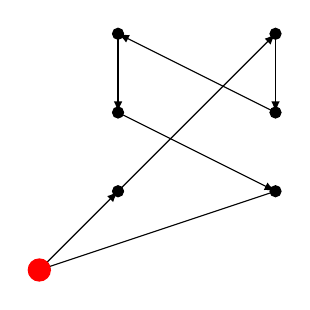
\begin{tikzpicture}
                \draw [black, -latex] (0, 0) -- (1, 1);
                \filldraw [black] (0, 0) circle (2pt);
                \draw [black, -latex] (1, 1) --(3, 3);
                \filldraw [black] (1, 1) circle (2pt);
                \draw [black, -latex] (3, 3) --(3, 2);
                \filldraw [black] (3, 3) circle (2pt);
                \draw [black, -latex] (3, 2) --(1, 3);
                \filldraw [black] (3, 2) circle (2pt);
                \draw [black, -latex] (1, 3) --(1, 2);
                \filldraw [black] (1, 3) circle (2pt);
                \draw [black, -latex] (1, 2) --(3, 1);
                \filldraw [black] (1, 2) circle (2pt);
                \draw [black, -latex] (3, 1) --(0, 0);
                \filldraw (3, 1) [black] circle (2pt);
                \filldraw [red] (0, 0) circle (4pt);
            \end{tikzpicture}
        \end{minipage}
        \begin{minipage}{0.3\linewidth}
            % Greedy
            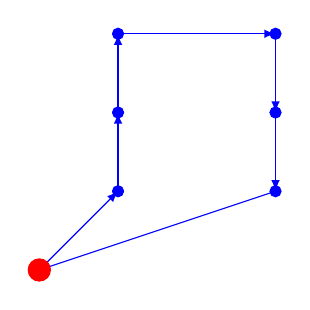
\begin{tikzpicture}
                \draw [blue, -latex] (0, 0) -- (1, 1);
                \filldraw [blue] (0, 0) circle (2pt);
                \draw [blue, -latex] (1, 1) --(1, 2);
                \filldraw [blue] (1, 1) circle (2pt);
                \draw [blue, -latex] (1, 2) --(1, 3);
                \filldraw [blue] (1, 2) circle (2pt);
                \draw [blue, -latex] (1, 3) --(3, 3);
                \filldraw [blue] (1, 3) circle (2pt);
                \draw [blue, -latex] (3, 3) --(3, 2);
                \filldraw [blue] (3, 3) circle (2pt);
                \draw [blue, -latex] (3, 2) --(3, 1);
                \filldraw [blue] (3, 2) circle (2pt);
                \draw [blue, -latex] (3, 1) --(0, 0);
                \filldraw (3, 1) [blue] circle (2pt);
                \filldraw [red] (0, 0) circle (4pt);
            \end{tikzpicture}
        \end{minipage}
        \begin{minipage}{0.3\linewidth}
            % opt2
            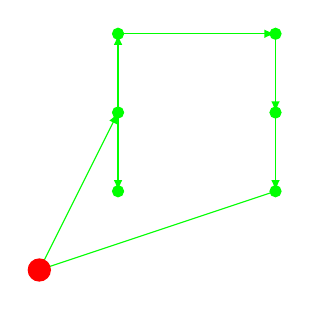
\begin{tikzpicture}
                \draw [green, -latex] (0, 0) -- (1, 2);
                \filldraw [green] (0, 0) circle (2pt);
                \draw [green, -latex] (1, 2) --(1, 1);
                \filldraw [green] (1, 2) circle (2pt);
                \draw [green, -latex] (1, 1) --(1, 3);
                \filldraw [green] (1, 1) circle (2pt);
                \draw [green, -latex] (1, 3) --(3, 3);
                \filldraw [green] (1, 3) circle (2pt);
                \draw [green, -latex] (3, 3) --(3, 2);
                \filldraw [green] (3, 3) circle (2pt);
                \draw [green, -latex] (3, 2) --(3, 1);
                \filldraw [green] (3, 2) circle (2pt);
                \draw [green, -latex] (3, 1) --(0, 0);
                \filldraw (3, 1) [green] circle (2pt);
                \filldraw [red] (0, 0) circle (4pt);
            \end{tikzpicture}
        \end{minipage}
    \end{figure}

    \subsection{Multiple Traveling Salesmen Problem}
    \label{subsection:Multiple_Traveling_Salesmen_Problem}
    
    Optimizing multiple routes simultaneously extends our 
    Traveling Salesman Problem to the Multiple Travelling 
    Salesman Problem (MTSP). Seeing how computationally 
    expensive our initial opt2 algorithm was in section 
    \ref{subsection:Traveling_Salesman_Problem} , one can imagine how much greater 
    this costs would become for an algorithm that optimized 
    multiple routes simeltaneously. For this reason, and 
    others we will, aim to optimize only two routes at 
    once. As mentioned in section \ref{subsection:Traveling_Salesman_Problem} we can achieve this 
    by extending the opt-2 heuristic to multiple routes, as seen in Listing \ref{lst:opt2_multi_algorithm}
    
    % fix this work like a numbered list
    \begin{lstlisting} [
        caption=opt2 Multi Algorithm,
        label={lst:opt2_multi_algorithm}
    ]
For all possible segments for both routes
    swap both routes with the following variations:
        1. Reverse route 1 then swap
        2. Reverse route 2 then swap
        3. Just swap
        4. Reverse both routes then swap
    If the distance from any of the variations is improved
        keep the modification.\end{lstlisting}
    
    
    As mentioned previously in this section, 
    we can expect the time complexity of this algorithm 
    to be larger than that of the single route opt-2 algorithm. 
    The multi-path opt-2 algorithm uses four for-loops 
    (two for each route). Further, at each iteration 
    of the innermost loop, we call our reverse and swap 
    methods several times. Both methods have a time
     complexity of O(n) (where n is the number of 
     addresses in each route). Since those methods 
     are called in total nine times, the time complexity 
     of the innermost loops is O(9n) which simplifies to O(n).
     Consequently, when we consider our four for-loops 
     the overall time complexity becomes O(n\textsuperscript5)
     \footnote{Futhermore, the time complexity would be 
     O(m\textsuperscript5+n\textsuperscript5) If we consider 
     routes of differing lengths m and n}. It’s important to 
     note that the time complexity of this algorithm 
     can also be improved, but at a cost. For example, 
     two for-loops are created to account for total 
     possible starting and ending of each segment per 
     route. To improve runtime, we could simply give 
     each segment a fixed length, thereby reducing 
     the time complexity to O(n\textsuperscript3). However, 
     this comes at the cost of accuracy, as our algorithm 
     may ignore more optimal solutions due to this constraint. 
     Therefore, therein lies a tradeoff between accuracy and 
     efficiency that we must consider when choosing which 
     approach/algorithm to use. The figures below demonstrate 
     this tradeoff visually:
     \begin{figure}[h]
        \caption{**include graph. Caption 1: Multi-path opt-2 algorithm with permitting swaps of fixed segment length 3 ( O(n\textsuperscript3) )
        Caption 2: Multi-path opt-2 algorithm with permitting swaps of varied segment lengths ( O(n\textsuperscript5) ). ****
        }
    \end{figure}

    In prioritizing accuracy, we will choose to pay the computational costs and use a multi-path-op2 algorithm that swaps segments of varied lengths efficient mulit-path opt-2 algorithm may require. Additionally, we can also choose to use this algorithm to optimize two routes belonging to a single driver (that is, spread over two different days). In this case, we may also want to consider optimizing for the total distance traveled by both routes, rather than the \emph{individual} distance traveled by both routes. The figures below demonstrate how this subtle change in constraints produces dramatically different results:
    \begin{figure}[h]
        \caption{*** include graphs use example test case from book: 
        Caption 1: Multi-path opt-2 algorithm optimizing for the individual distance traveled by both routes. 
        Caption 2: Multi-path opt-2 algorithm optimizing for the total distance traveled by both routes. 
        ****INCLUDE INDIVIDUAL LENGTHS  AND TOTAL DISTANCES FOR EACH CAPTION
        }
    \end{figure}
    
    Notice how in Figure XXX (caption 2) we achieve a smaller total distance at the expense of increasing the individual distance of route XXX. Whereas in Figure XXX (caption 1) we optimize for the individual distances of each route at the expense of having a larger total distance (from taking the sum of both routes). As a result, it seems we may want to optimize for total distance and individual distance on a case-by-case basis. For example, in the scenario of scheduling routes for multiple (in this case two) Amazon truck drivers it may seem more logical to optimize for individual distances. This is because having lopsided routes similar to that shown in Figure XXX (caption 1) can lead to undelivered packages (in the event that one route is so long all points cannot be visited in a single shift of work). Conversely, in the scenario that we were trying to optimize two routes belonging to the same truck driver, it seems more logical to optimize for total distance traveled across both routes (although this is assuming delivery timing is not a factor)\footnote{this is because swapping segments containing different delivery times would lead to some packages being delivered early while others being delivered too late. We don't mind early deliveries, but late deliveries are unacceptable}. For our final product, we will explore ways to utilize the multi-path opt2 algorithm (including the others previously discussed) in optimzing truck routes for drivers.  
    \newline{}\newline{}
    Talk about how swap algorithm works. Figure \ref{figure:swapdemo} provides a simple example of how this algorithm improves the total distance. (Now prove it with data! What are the distances before and after?) ALSO: Talk about how the gray and black Addresses are symmetrical, but the trucks take different Routes. Is this okay, or does one or both of them need to go through greedy/opt2???

    \begin{figure}[h]
        \caption{Two Routes exchange Addresses to optimize their distances.}
        \label{figure:swapdemo}
        \begin{minipage}{0.45\linewidth}
            % Unswapped
            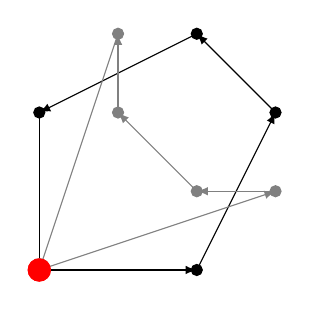
\begin{tikzpicture}
                % Route 1
                \draw [black, -latex] (0, 0) -- (2, 0);
                \filldraw [black] (0, 0) circle (2pt);
                \draw [black, -latex] (2, 0) --(3, 2);
                \filldraw [black] (2, 0) circle (2pt);
                \draw [black, -latex] (3, 2) --(2, 3);
                \filldraw [black] (3, 2) circle (2pt);
                \draw [black, -latex] (2, 3) --(0, 2);
                \filldraw [black] (2, 3) circle (2pt);
                \draw [black, -latex] (0, 2) --(0, 0);
                \filldraw (0, 2) [black] circle (2pt);
                \filldraw [red] (0, 0) circle (4pt);
                % Route 2
                \draw [gray, -latex] (0, 0) -- (3, 1);
                \filldraw [gray] (0, 0) circle (2pt);
                \draw [gray, -latex] (3, 1) --(2, 1);
                \filldraw [gray] (3, 1) circle (2pt);
                \draw [gray, -latex] (2, 1) --(1, 2);
                \filldraw [gray] (2, 1) circle (2pt);
                \draw [gray, -latex] (1, 2) --(1, 3);
                \filldraw [gray] (1, 2) circle (2pt);
                \draw [gray, -latex] (1, 3) --(0, 0);
                \filldraw (1, 3) [gray] circle (2pt);
                \filldraw [red] (0, 0) circle (4pt);
            \end{tikzpicture}
        \end{minipage}
        \begin{minipage}{0.45\linewidth}
            % Swapped
            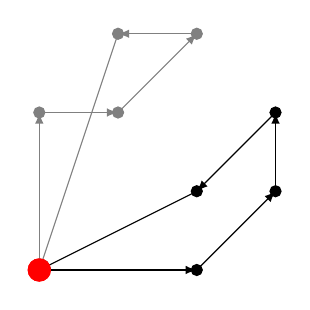
\begin{tikzpicture}
                % Route 1
                \draw [black, -latex] (0, 0) -- (2, 0);
                \filldraw [black] (0, 0) circle (2pt);
                \draw [black, -latex] (2, 0) --(3, 1);
                \filldraw [black] (2, 0) circle (2pt);
                \draw [black, -latex] (3, 1) --(3, 2);
                \filldraw [black] (3, 1) circle (2pt);
                \draw [black, -latex] (3, 2) --(2, 1);
                \filldraw [black] (3, 2) circle (2pt);
                \draw [black, -latex] (2, 1) --(0, 0);
                \filldraw (2, 1) [black] circle (2pt);
                \filldraw [red] (0, 0) circle (4pt);
                % Route 2
                \draw [gray, -latex] (0, 0) -- (0, 2);
                \filldraw [gray] (0, 0) circle (2pt);
                \draw [gray, -latex] (0, 2) --(1, 2);
                \filldraw [gray] (0, 2) circle (2pt);
                \draw [gray, -latex] (1, 2) --(2, 3);
                \filldraw [gray] (1, 2) circle (2pt);
                \draw [gray, -latex] (2, 3) --(1, 3);
                \filldraw [gray] (2, 3) circle (2pt);
                \draw [gray, -latex] (1, 3) --(0, 0);
                \filldraw (1, 3) [gray] circle (2pt);
                \filldraw [red] (0, 0) circle (4pt);
            \end{tikzpicture}
        \end{minipage}
    \end{figure}

    \subsection{Developing the Final Product}
    \label{subsection:Developing_the_Final_Product}
    After our team implemented our solutions to the Single and Multiple Traveling Salesman Problems, we decided to explore dynamicism by constructing a simplified route allocator for a delivery company. Every morning, a regional fulfilment center recives a list of orders to fulfill, corresponding to packages available onsite. It invokes our program, which combines these with unfulfilled orders from the previous day, and delegates them amongst a predetermined number of trucks. The \verb|Route|s are then optimized individually and between one another. At this point, their distances are measured. If a \verb|Route| exceeds a predetermined distance limit, \verb|Address|es are removed from the \verb|Route| based on their \verb|deliver_by| due date, until it falls within an acceptable length. The delivery routes are then exported to documents for the drivers, the unfulfilled orders are saved to a file which overwrites the old one, and performance statistics are compiled into a report for management.

    All of the tasks to be completed before the start of a business day are modularized in a single function. It requires parameters specifying input and output file locations, the number of trucks available, the maximum permissible route distance, the hub address, and a boolean which allows the user to specify if data should be output from intermediate optimization steps. Most of the harder tasks of the simulation have already been solved in our library. This even includes the repetitive tasks of reading or exporting a \verb|Route| or \verb|AddressList| from or to a file, based on a given file path string. To demonstrate this program, we constructed a simulation with pre-generated daily orders spanning several days. The results of this simulation are discussed in Section \ref{section:Results}.

    \section{Results}
    \label{section:Results}
    % Pretty pictures and tables go here. Describe each situation being displayed and talk about what they mean, e.g. is it the optimal solution? Good enough? Is there a tradeoff between time to execute and quality of results?

    % Hmm, maybe insert a table comparing number of nodes/trucks to program execution time. What rate does it increase at $(O(n), O(n^2), \&c.)$

    For our main simulation, we generated randomized order data spanning 9 days. Each day has 18 orders with coordinates spanning from 0 to 10 excluding the hub, i.e. $\{ (i, j) \in \mathbb{Z}^2 | 0 \leq i \leq 10 \cap 0 \leq j \leq 10\} - \{ (0, 0)\}$. Delivery due dates range from 1 to 7 days after the order was generated. For this test, 3 trucks were used, and the distance limit was set to 35.0 for each truck. Our program took 795 milliseconds to execute locally, and XXXXXX milliseconds on the ISP machine. The resulting outputs, spread across over 100 data files, would be quite tedious to present in full in this report, so the results will be condensed into tables and figures. To view samples of each form of output, please refer to Appendix \ref{appendix:Sample_Output_Files}.

    The first thing to consider from the results is whether the optimization performed as expected. As seen in Figure \ref{figure:day1opt}, stops are exchanged within and between truck routes until they all take efficient paths. Since no orders were left undelivered on Day 1, all of the Addresses are still present afterwards. This can be verified for the other days as well.

    \begin{figure}[h]
        \caption{Day 1 Optimization, Before and After}
        \label{figure:day1opt}
        \begin{minipage}{0.45\linewidth}
            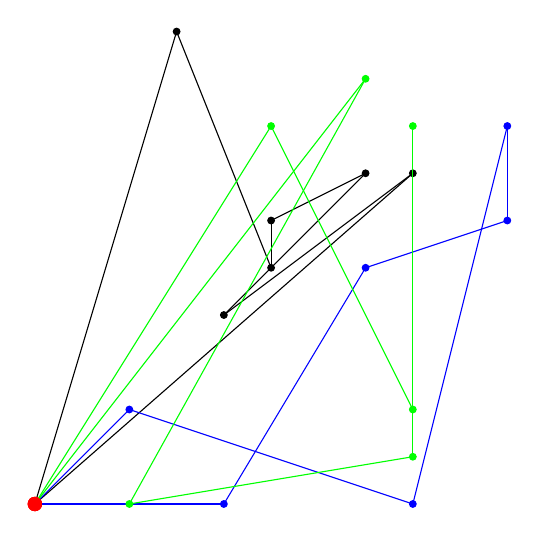
\begin{tikzpicture}[scale=0.6]
                % Truck 1
                \draw [black] (0, 0) -- (8, 7);
                \filldraw [black] (0, 0) circle (2pt);
                \draw [black] (8, 7) --(4, 4);
                \filldraw [black] (8, 7) circle (2pt);
                \draw [black] (4, 4) --(7, 7);
                \filldraw [black] (4, 4) circle (2pt);
                \draw [black] (7, 7) --(5, 6);
                \filldraw [black] (7, 7) circle (2pt);
                \draw [black] (5, 6) --(5, 5);
                \filldraw [black] (5, 6) circle (2pt);
                \draw [black] (5, 5) --(3, 10);
                \filldraw [black] (5, 5) circle (2pt);
                \draw [black] (3, 10) --(0, 0);
                \filldraw (3, 10) [black] circle (2pt);
                \filldraw [red] (0, 0) circle (4pt);
                % Truck 2
                \draw [blue] (0, 0) -- (4, 0);
                \filldraw [blue] (0, 0) circle (2pt);
                \draw [blue] (4, 0) --(7, 5);
                \filldraw [blue] (4, 0) circle (2pt);
                \draw [blue] (7, 5) --(10, 6);
                \filldraw [blue] (7, 5) circle (2pt);
                \draw [blue] (10, 6) --(10, 8);
                \filldraw [blue] (10, 6) circle (2pt);
                \draw [blue] (10, 8) --(8, 0);
                \filldraw [blue] (10, 8) circle (2pt);
                \draw [blue] (8, 0) --(2, 2);
                \filldraw [blue] (8, 0) circle (2pt);
                \draw [blue] (2, 2) --(0, 0);
                \filldraw (2, 2) [blue] circle (2pt);
                \filldraw [red] (0, 0) circle (4pt);
                % Truck 3
                \draw [green] (0, 0) -- (5, 8);
                \filldraw [green] (0, 0) circle (2pt);
                \draw [green] (5, 8) --(8, 2);
                \filldraw [green] (5, 8) circle (2pt);
                \draw [green] (8, 2) --(8, 8);
                \filldraw [green] (8, 2) circle (2pt);
                \draw [green] (8, 8) --(8, 1);
                \filldraw [green] (8, 8) circle (2pt);
                \draw [green] (8, 1) --(2, 0);
                \filldraw [green] (8, 1) circle (2pt);
                \draw [green] (2, 0) --(7, 9);
                \filldraw [green] (2, 0) circle (2pt);
                \draw [green] (7, 9) --(0, 0);
                \filldraw (7, 9) [green] circle (2pt);
                \filldraw [red] (0, 0) circle (4pt);
            \end{tikzpicture}
        \end{minipage}
        \begin{minipage}{0.45\linewidth}
            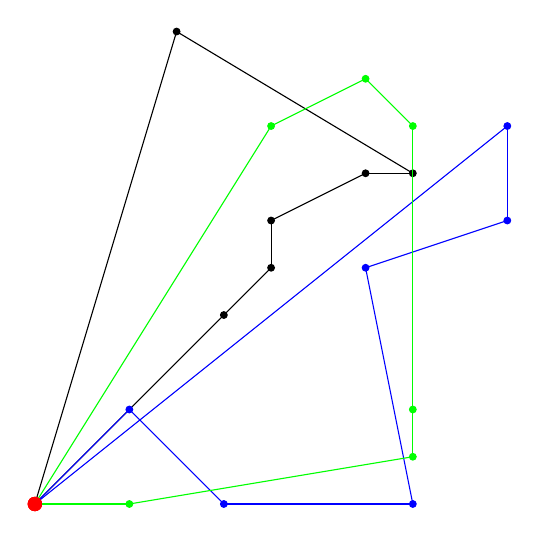
\begin{tikzpicture}[scale=0.6]
                % Truck 1
                \draw [black] (0, 0) -- (4, 4);
                \filldraw [black] (0, 0) circle (2pt);
                \draw [black] (4, 4) --(5, 5);
                \filldraw [black] (4, 4) circle (2pt);
                \draw [black] (5, 5) --(5, 6);
                \filldraw [black] (5, 5) circle (2pt);
                \draw [black] (5, 6) --(7, 7);
                \filldraw [black] (5, 6) circle (2pt);
                \draw [black] (7, 7) --(8, 7);
                \filldraw [black] (7, 7) circle (2pt);
                \draw [black] (8, 7) --(3, 10);
                \filldraw [black] (8, 7) circle (2pt);
                \draw [black] (3, 10) --(0, 0);
                \filldraw (3, 10) [black] circle (2pt);
                \filldraw [red] (0, 0) circle (4pt);
                % Truck 2
                \draw [blue] (0, 0) -- (2, 2);
                \filldraw [blue] (0, 0) circle (2pt);
                \draw [blue] (2, 2) --(4, 0);
                \filldraw [blue] (2, 2) circle (2pt);
                \draw [blue] (4, 0) --(8, 0);
                \filldraw [blue] (4, 0) circle (2pt);
                \draw [blue] (8, 0) --(7, 5);
                \filldraw [blue] (8, 0) circle (2pt);
                \draw [blue] (7, 5) --(10, 6);
                \filldraw [blue] (7, 5) circle (2pt);
                \draw [blue] (10, 6) --(10, 8);
                \filldraw [blue] (10, 6) circle (2pt);
                \draw [blue] (10, 8) --(0, 0);
                \filldraw (10, 8) [blue] circle (2pt);
                \filldraw [red] (0, 0) circle (4pt);
                % Truck 3
                \draw [green] (0, 0) -- (2, 0);
                \filldraw [green] (0, 0) circle (2pt);
                \draw [green] (2, 0) --(8, 1);
                \filldraw [green] (2, 0) circle (2pt);
                \draw [green] (8, 1) --(8, 2);
                \filldraw [green] (8, 1) circle (2pt);
                \draw [green] (8, 2) --(8, 8);
                \filldraw [green] (8, 2) circle (2pt);
                \draw [green] (8, 8) --(7, 9);
                \filldraw [green] (8, 8) circle (2pt);
                \draw [green] (7, 9) --(5, 8);
                \filldraw [green] (7, 9) circle (2pt);
                \draw [green] (5, 8) --(0, 0);
                \filldraw (5, 8) [green] circle (2pt);
                \filldraw [red] (0, 0) circle (4pt);
            \end{tikzpicture}
        \end{minipage}
    \end{figure}

    Reports and data files can also be examined for their accuracy; refer to Listings \ref{lst:Sample_Data_File} and \ref{lst:Sample_TikZ_File} to see that they correspond to the black unsorted route. On the other hand, the job assignment in Listing \ref{lst:Sample_Job_Assignment} corresponds to the black sorted route, and the order numbers in the status report in Listing \ref{lst:Sample_Satus_Report} match the number of stops and distances of the sorted routes.

    From there, we can study the numbers provided in the status reports. The numbers are condensed into Table \ref{table:deliverystats}.

    \begin{table}[h]
        \centering
        \caption{Status Report Output Data}
        \label{table:deliverystats}
        \begin{tabular}{cccccccc}
            & \multicolumn{3}{c}{Delivered} && \multicolumn{3}{c}{Undelivered} \\
            & Early & On Time & Late && Not Due & Due Tomorrow & Overdue \\
            \cline{2-4} \cline{6-8}
            Day 1 & 18 & 0 & 0 && 0 & 0 & 0 \\
            Day 2 & 16 & 0 & 0 && 0 & 0 & 0 \\
            Day 3 &  &  &  &&  &  &  \\
            Day 4 &  &  &  &&  &  &  \\
            Day 5 &  &  &  &&  &  &  \\
            Day 6 &  &  &  &&  &  &  \\
            Day 7 &  &  &  &&  &  &  \\
            Day 8 &  &  &  &&  &  &  \\
            Day 9 &  &  &  &&  &  &  \\
        \end{tabular}
    \end{table}

    \subsection{Varying the Distance Limit}
    \label{}
    Note that if the distance limit dropped below $2 * 10 \sqrt{2} \approx 28.284$, then some orders would be forever out of range.

    \subsection{Varying the Number of Trucks Deployed}
    \label{subsection:Investigating_the_Number_of_Trucks_Deployed}
    One important question that a delivery company might want to consider is how many trucks to deploy on a given day. More trucks can cover a greater cumulative distance and deliver more orders, but 

    \subsection{Performance Data}
    go over execution time and stuff

    \section{Conclusion}
    \label{section:Conclusion}
    Talk about what we learned, how this all applies to industry, ideas to scale the problem up, ethics, \&c.

    Talk about how our simulation is flawed, e.g. address removal isn't intelligent (purely by due date); orders aren't held back to be grouped with later-arriving orders; after stops are removed, the routes arent re optimized; main simulation program isn't super flexible (e.g. to change document names, formattig, you have to go into the code; dat files have to be in a specific format, can't be a database); no UI for ease of use

    \appendix
    \section{Sample Output Files}
    \label{appendix:Sample_Output_Files}

    A variety of data files are used as inputs, intermediates, and outputs of our main program and scripts. They fall into 4 main categories. Data files like Listing \ref{lst:Sample_Data_File} are used to input Addresses into the program and save output Routes from the program. The example is clearly a Route, since it starts and ends at the same location, in this case, the origin. TikZ files like Listing \ref{lst:Sample_TikZ_File} are used to automate plotting figures with the TikZ package in \LaTeX . Job assignments like Listing \ref{lst:Sample_Job_Assignment} format Routes such that human drivers can read them. They also offer some statistics and custom messages. In this case, an affirmation is distributed to drivers to increase morale. Finally, status reports like Listing \ref{lst:Sample_Satus_Report} condense essential information like delivery numbers for managers to evaluate the hub's performance.

    \lstinputlisting[caption=Sample Data File, label={lst:Sample_Data_File}]{day1_truck1_v0.dat}

    \lstinputlisting[caption=Sample TikZ File, label={lst:Sample_TikZ_File}]{day1_truck1_v0.tikz}

    \lstinputlisting[caption=Sample Job Assignment, label={lst:Sample_Job_Assignment}]{day1_truck1.txt}

    \lstinputlisting[caption=Sample Status Report, label={lst:Sample_Satus_Report}]{day1_status.txt}

    \bibliographystyle{plain}
    \bibliography{ref}
\end{document}